\documentclass[12pt]{article}

% chinese fonts
\usepackage{ctex}

% table of contents
\usepackage{tocloft}
\setlength\cftbeforesecskip{.4em}
\setlength\cftbeforesubsecskip{.4em}

% math fonts
\usepackage{amsmath}
\usepackage{amsthm}
\usepackage{amssymb}
\usepackage{bm}

% figures
\usepackage{tikz}
\usepackage{graphicx}
\graphicspath{{./figures/}}

% tables
\usepackage{tabularx}
\usepackage{booktabs}
\usepackage{multirow}
\usepackage[figuresright]{rotating}
\usepackage{longtable}

\usepackage{enumerate}

% codes
\usepackage{listings}
\lstset{language     = Matlab,
        basicstyle   = \ttfamily,
        keywordstyle = \color{cyan},
        rulecolor    = \color{black},
        commentstyle = \color{green},
        keepspaces   = true,
        tabsize      = 4,
}

% hyperlinks
\usepackage{hyperref}
\hypersetup{
  breaklinks,
  colorlinks = true,
  citecolor  = blue,
  linkcolor  = red,
  urlcolor   = magenta,
}

% algorithms
% algorithms
\makeatletter
  \newif\if@restonecol
\makeatother
\let\algorithm\relax
\let\endalgorithm\relax
\usepackage[linesnumbered,ruled,lined]{algorithm2e}
\usepackage{algpseudocode}
\renewcommand{\algorithmicrequire}{\textbf{Input:}}  % Use Input in the format of Algorithm
\renewcommand{\algorithmicensure}{\textbf{Output:}} % Use Output in the format of Algorithm

% bibliography
\usepackage[sort&compress,numbers]{natbib}

% About:  Macros for Vector, Matrix, Tensor, Math Operator and Misc
% Author: Jingxuan Yang

% vectors
\newcommand{\va}{\bm{a}}       \newcommand{\vah}{\hat{\bm{a}}}        \newcommand{\ah}{\hat{a}}    \newcommand{\vat}{\tilde{\bm{a}}}       \newcommand{\at}{\tilde{a}}
\newcommand{\vb}{\bm{b}}       \newcommand{\vbh}{\hat{\bm{b}}}        \newcommand{\bh}{\hat{b}}    \newcommand{\vbt}{\tilde{\bm{b}}}       \newcommand{\bt}{\tilde{b}}
\newcommand{\vc}{\bm{c}}       \newcommand{\vch}{\hat{\bm{c}}}        \newcommand{\ch}{\hat{c}}    \newcommand{\vct}{\tilde{\bm{c}}}       \newcommand{\ct}{\tilde{c}}
\newcommand{\vd}{\bm{d}}       \newcommand{\vdh}{\hat{\bm{d}}}        \newcommand{\dhat}{\hat{d}}  \newcommand{\vdt}{\tilde{\bm{d}}}       \newcommand{\dt}{\tilde{d}}
\newcommand{\ve}{\bm{e}}       \newcommand{\veh}{\hat{\bm{e}}}        \newcommand{\eh}{\hat{e}}    \newcommand{\vet}{\tilde{\bm{e}}}       \newcommand{\et}{\tilde{e}}
\newcommand{\vf}{\bm{f}}       \newcommand{\vfh}{\hat{\bm{f}}}        \newcommand{\fh}{\hat{f}}    \newcommand{\vft}{\tilde{\bm{f}}}       \newcommand{\ft}{\tilde{f}}
\newcommand{\vg}{\bm{g}}       \newcommand{\vgh}{\hat{\bm{g}}}        \newcommand{\gh}{\hat{g}}    \newcommand{\vgt}{\tilde{\bm{g}}}       \newcommand{\gt}{\tilde{g}}
\newcommand{\vech}{\bm{h}}     \newcommand{\vhh}{\hat{\bm{h}}}        \newcommand{\hh}{\hat{h}}    \newcommand{\vht}{\tilde{\bm{h}}}       \newcommand{\htild}{\tilde{h}}
\newcommand{\vi}{\bm{i}}       \newcommand{\vih}{\hat{\bm{i}}}        \newcommand{\ih}{\hat{i}}    \newcommand{\vit}{\tilde{\bm{i}}}       \newcommand{\itild}{\tilde{i}}
\newcommand{\vj}{\bm{j}}       \newcommand{\vjh}{\hat{\bm{j}}}        \newcommand{\jh}{\hat{j}}    \newcommand{\vjt}{\tilde{\bm{j}}}       \newcommand{\jt}{\tilde{j}}
\newcommand{\vk}{\bm{k}}       \newcommand{\vkh}{\hat{\bm{k}}}        \newcommand{\kh}{\hat{k}}    \newcommand{\vkt}{\tilde{\bm{k}}}       \newcommand{\kt}{\tilde{k}}
\newcommand{\vl}{\bm{l}}       \newcommand{\vlh}{\hat{\bm{l}}}        \newcommand{\lh}{\hat{l}}    \newcommand{\vlt}{\tilde{\bm{l}}}       \newcommand{\lt}{\tilde{l}}
\newcommand{\vm}{\bm{m}}       \newcommand{\vmh}{\hat{\bm{m}}}        \newcommand{\mh}{\hat{m}}    \newcommand{\vmt}{\tilde{\bm{m}}}       \newcommand{\mt}{\tilde{m}}
\newcommand{\vn}{\bm{n}}       \newcommand{\vnh}{\hat{\bm{n}}}        \newcommand{\nh}{\hat{n}}    \newcommand{\vnt}{\tilde{\bm{n}}}       \newcommand{\nt}{\tilde{n}}
\newcommand{\vo}{\bm{o}}       \newcommand{\voh}{\hat{\bm{o}}}        \newcommand{\oh}{\hat{o}}    \newcommand{\vot}{\tilde{\bm{o}}}       \newcommand{\ot}{\tilde{o}}
\newcommand{\vp}{\bm{p}}       \newcommand{\vph}{\hat{\bm{p}}}        \newcommand{\ph}{\hat{p}}    \newcommand{\vpt}{\tilde{\bm{p}}}       \newcommand{\pt}{\tilde{p}}
\newcommand{\vq}{\bm{q}}       \newcommand{\vqh}{\hat{\bm{q}}}        \newcommand{\qh}{\hat{q}}    \newcommand{\vqt}{\tilde{\bm{q}}}       \newcommand{\qt}{\tilde{q}}
\newcommand{\vr}{\bm{r}}       \newcommand{\vrh}{\hat{\bm{r}}}        \newcommand{\rh}{\hat{r}}    \newcommand{\vrt}{\tilde{\bm{r}}}       \newcommand{\rt}{\tilde{r}}
\newcommand{\vs}{\bm{s}}       \newcommand{\vsh}{\hat{\bm{s}}}        \newcommand{\sh}{\hat{s}}    \newcommand{\vst}{\tilde{\bm{s}}}       \newcommand{\st}{\tilde{s}}
\newcommand{\vt}{\bm{t}}       \newcommand{\vth}{\hat{\bm{t}}}        \newcommand{\that}{\hat{t}}  \newcommand{\vtt}{\tilde{\bm{t}}}       \newcommand{\ttil}{\tilde{t}}
\newcommand{\vu}{\bm{u}}       \newcommand{\vuh}{\hat{\bm{u}}}        \newcommand{\uh}{\hat{u}}    \newcommand{\vut}{\tilde{\bm{u}}}       \newcommand{\ut}{\tilde{u}}
\newcommand{\vv}{\bm{v}}       \newcommand{\vvh}{\hat{\bm{v}}}        \newcommand{\vh}{\hat{v}}    \newcommand{\vvt}{\tilde{\bm{v}}}       \newcommand{\vtild}{\tilde{v}}
\newcommand{\vw}{\bm{w}}       \newcommand{\vwh}{\hat{\bm{w}}}        \newcommand{\wh}{\hat{w}}    \newcommand{\vwt}{\tilde{\bm{w}}}       \newcommand{\wt}{\tilde{w}}
\newcommand{\vx}{\bm{x}}       \newcommand{\vxh}{\hat{\bm{x}}}        \newcommand{\xh}{\hat{x}}    \newcommand{\vxt}{\tilde{\bm{x}}}       \newcommand{\xt}{\tilde{x}}
\newcommand{\vy}{\bm{y}}       \newcommand{\vyh}{\hat{\bm{y}}}        \newcommand{\yh}{\hat{y}}    \newcommand{\vyt}{\tilde{\bm{y}}}       \newcommand{\yt}{\tilde{y}}
\newcommand{\vz}{\bm{z}}       \newcommand{\vzh}{\hat{\bm{z}}}        \newcommand{\zh}{\hat{z}}    \newcommand{\vzt}{\tilde{\bm{z}}}       \newcommand{\zt}{\tilde{z}}

\newcommand{\valpha}{\bm{\alpha}}
\newcommand{\vbeta}{\bm{\beta}}
\newcommand{\vgamma}{\bm{\gamma}}
\newcommand{\vtheta}{\bm{\theta}}
\newcommand{\vlambda}{\bm{\lambda}}
\newcommand{\vmu}{\bm{\mu}}
\newcommand{\vomega}{\bm{\omega}}
\newcommand{\vxi}{\bm{\xi}}
\newcommand{\veta}{\bm{\eta}}
\newcommand{\vvarepsilon}{\bm{\varepsilon}}

\newcommand{\mSigma}{\bm{\Sigma}}
\newcommand{\mLambda}{\bm{\Lambda}}

\newcommand{\Ac}{\mathcal{A}}
\newcommand{\Fc}{\mathcal{F}}
\newcommand{\Xc}{\mathcal{X}}
\newcommand{\Yc}{\mathcal{Y}}
\newcommand{\Zc}{\mathcal{Z}}
\newcommand{\Gc}{\mathcal{G}}
\newcommand{\Hc}{\mathcal{H}}
\newcommand{\Dc}{\mathcal{D}}
\newcommand{\Cc}{\mathcal{C}}
\newcommand{\Rc}{\mathcal{R}}
\newcommand{\Nc}{\mathcal{N}}

% matrices
\newcommand{\ma}{\bm{A}}
\newcommand{\mb}{\bm{B}}
\newcommand{\mc}{\bm{C}}
\newcommand{\md}{\bm{D}}
\newcommand{\mE}{\bm{E}}
\newcommand{\mf}{\bm{F}}
\newcommand{\mg}{\bm{G}}
\newcommand{\mH}{\bm{H}}
\newcommand{\mi}{\bm{I}}
\newcommand{\mj}{\bm{J}}
\newcommand{\mk}{\bm{K}}
\newcommand{\ml}{\bm{L}}
\newcommand{\mM}{\bm{M}}
\newcommand{\mn}{\bm{N}}
\newcommand{\mO}{\bm{O}}
\newcommand{\mP}{\bm{P}}
\newcommand{\mq}{\bm{Q}}
\newcommand{\mr}{\bm{R}}
\newcommand{\ms}{\bm{S}}
\newcommand{\mT}{\bm{T}}
\newcommand{\mU}{\bm{U}}
\newcommand{\mv}{\bm{V}}
\newcommand{\mw}{\bm{W}}
\newcommand{\mx}{\bm{X}}
\newcommand{\my}{\bm{Y}}
\newcommand{\mz}{\bm{Z}}

% tensors
\newcommand{\tp}{\mathsf{P}}
\newcommand{\tu}{\mathsf{U}}
\newcommand{\tx}{\mathsf{X}}
\newcommand{\ty}{\mathsf{Y}}
\newcommand{\tz}{\mathsf{Z}}
\newcommand{\tw}{\mathsf{W}}

% norms
\newcommand{\mynorm}[2]{\| {#1} \|_{#2}}
\newcommand{\norm}[2]{\mynorm{#1}{#2}}
\newcommand{\bignorm}[2]{\left\| {#1} \right\|_{#2}}
\newcommand{\norml}[1]{\mynorm{#1}{1}}
\newcommand{\bignorml}[1]{\bignorm{#1}{1}}
\newcommand{\infnorm}[1]{\mynorm{#1}{\infty}}
\newcommand{\biginfnorm}[1]{\bignorm{#1}{\infty}}
\newcommand{\oneinf}{\ell_{1,\infty}}
\newcommand{\onetwo}{\ell_{1,2}}
\newcommand{\oneinfnorm}[1]{\mynorm{#1}{1,\infty}}
\newcommand{\bigoneinf}[1]{\bignorm{#1}{1,\infty}}
\newcommand{\onetwonorm}[1]{\mynorm{#1}{1,2}}
\newcommand{\bigonetwo}[1]{\bignorm{#1}{1,2}}
\newcommand{\enorm}[1]{\mynorm{#1}{2}}
\newcommand{\bigenorm}[1]{\bignorm{#1}{2}}
\newcommand{\znorm}[1]{\mynorm{#1}{0}}
\newcommand{\bigznorm}[1]{\bignorm{#1}{0}}
\newcommand{\frob}[1]{\|{#1}\|_{\text{F}}}
\newcommand{\bigfrob}[1]{\bignorm{#1}{\text{F}}}
\newcommand{\grpnorm}[2]{\norm{#1}{\text{Gr}(#2)}}

% math operators
\DeclareMathOperator*{\argmin}{argmin}
\DeclareMathOperator*{\argmax}{argmax}
\DeclareMathOperator{\divg}{div}
\DeclareMathOperator{\dom}{dom}
\DeclareMathOperator{\interior}{int}
\DeclareMathOperator{\ri}{ri}
\DeclareMathOperator{\sgn}{sgn}
\DeclareMathOperator{\trace}{tr}
\DeclareMathOperator{\diag}{diag}
\DeclareMathOperator{\rank}{rank}
\DeclareMathOperator{\range}{Range}
\DeclareMathOperator{\vect}{vec}
\DeclareMathOperator{\prox}{prox}
\DeclareMathOperator{\intr}{int}
\DeclareMathOperator{\relint}{ri}
\DeclareMathOperator{\image}{Im}
\DeclareMathOperator{\kernal}{Ker}
\let\span\relax
\DeclareMathOperator{\span}{Span}
\DeclareMathOperator{\var}{Var}
\DeclareMathOperator{\cov}{Cov}

% misc
\newcommand{\gs}{\geqslant}
\newcommand{\ls}{\leqslant}
\newcommand{\set}[1]{\left\{ {#1}\right\}}

\newcommand{\defeq}{\ \stackrel{\text{def}}{=}\ }
\newcommand{\ip}[2]{\left\langle#1, #2\right\rangle}
\newcommand{\reals}{\mathbb{R}}
\newcommand{\complex}{\mathbb{C}}
\newcommand{\E}{\mathbb{E}}
\newcommand{\hop}{\mathrm{H}}
\renewcommand{\i}{\mathrm{i}}
\renewcommand{\j}{\mathrm{j}}
\newcommand{\half}{\frac{1}{2}}

\newtheorem{theorem}{Theorem}
\newtheorem{lemma}[theorem]{Lemma}
\newtheorem{proposition}[theorem]{Proposition}
\newtheorem{remark}[theorem]{Remark}
\newtheorem{corollary}[theorem]{Corollary}
\newtheorem{definition}[theorem]{Definition}


\setlength{\oddsidemargin}{-0.25 in}
\setlength{\evensidemargin}{-0.25 in} 
\setlength{\topmargin}{-0.25in} 
\setlength{\textwidth}{7 in} 
\setlength{\textheight}{8.9 in}
\setlength{\headsep}{0.25 in} 
% \setlength{\parindent}{0 in}
\setlength{\parskip}{0.1 in}

\newcommand{\homework}[5]{
  \pagestyle{myheadings} 
  \thispagestyle{plain}
  \newpage
  \setcounter{page}{1}
  \noindent
  \begin{center}
    \framebox{ 
      \vbox{
        \vspace{2mm} 
        \hbox to 6.28in { {\bf
        Matrix Analysis and Applications (Autumn 2022) \hfill Final Project} }
        \vspace{6mm} 
        \hbox to 6.28in { {\Large \hfill #1 \hfill} }
        \vspace{6mm} 
        \hbox to 6.28in { {\it Lecturer: #2 \hfill} }
        \vspace{2mm} 
        \hbox to 6.28in { {\it Student: #3 \hfill} }
        \vspace{2mm} 
        \hbox to 6.28in { {\it \hspace*{15mm} #4 \hfill} }
        \vspace{2mm} 
      } 
    }
  \end{center}
  \markboth{#1}{#1} 
  \vspace*{4mm} 
}

\begin{document}

\homework{综合课题研究}{Feng Chen \hspace{10mm} {\tt chenfeng@mail.tsinghua.edu.cn}}{Jingxuan Yang \hspace{4mm} {\tt yangjx20@mails.tsinghua.edu.cn} }{Zewei Dong \hspace{9.9mm} {\tt dzw22@mails.tsinghua.edu.cn}}

\renewcommand{\abstractname}{\large 摘~~要}
\begin{abstract}

\normalsize

\hspace*{1mm} 图像数据的低秩矩阵恢复是计算机视觉与模式识别任务的重要研究问题. 本文针对低秩矩阵恢复问题进行探究, 主要研究了鲁棒主成分分析算法以及矩阵补全算法. 针对鲁棒主成分分析算法, 给出了基于梯度下降算法的通用求解方法, 并基于 Adam 算法进行优化, 然后给出了 3 种特殊优化算法: SVT, APG 与 ALM. 针对矩阵补全问题, 给出了矩阵补全问题的数学模型, 以及 4 种具体求解算法: SVT, ADMM, ALS, NTK. 本文对上述算法在图像数据集上的效果进行了测试, 结果表明 PCA 算法的求解时间最短, 但是效果比较一般, 鲁棒主成分分析算法的效果更好, 但是耗时普遍较长, 其中 SVT 算法的用时较短且取得了相对更好的效果; 矩阵补全算法也可以实现低秩矩阵恢复, ADMM 和 SVT 算法的效果均比较好但用时较长, CNTK 算法与 EigenPro 联合使用既用时少又效果好. 本文还对不同超参数的实验结果进行了测试和分析. 代码开源地址: \href{https://github.com/jingxuanyang/LowRankMatrixRestoration}{https://github.com/jingxuanyang/LowRankMatrixRestoration}.

\vspace{13.5pt}
\textbf{关键词}: 低秩矩阵恢复; 鲁棒主成分分析; 矩阵补全

\end{abstract}

\newpage
\tableofcontents

\section{引言}

在计算机视觉与模式识别任务中, 通常都假设观测数据近似存在于一个低维的子空间下. 为找出这样的子空间, 经典的主成分分析 (Principal Component Analysis, PCA) \cite{abdi2010principal} 方法假定数据受到较小的高斯噪声污染, 即数据 $\mM\in\reals^{m\times n}$ 由一个低秩矩阵 $\ml\in\reals^{m\times n}$ 和一个独立同分布的高斯噪声矩阵 $\ms\in\reals^{m\times n}$ 构成. 当给定超参数 $r\in\mathbb{N}_{>0}$ 时, 该任务可以建模为如下的优化问题: 
\begin{equation}
  \begin{aligned}
    &\min_{\ml,\ms}~\|\ms\|_{\text{F}} \\
    &~\text{s.t.}~\rank(\ml)\leqslant r,\\
    &\qquad \mM=\ml+\ms.
  \end{aligned}
\end{equation}

然而在实际应用中, 若出现较高幅度的尖锐噪声或严重的离群点时, PCA 的性能会受到很大的影响. 而另一方面, 当噪声矩阵 $\ms$ 足够稀疏时, 原始的低秩矩阵仍然可能被恢复 \cite{shi2013low}. 该任务可以建模为如下的优化问题: 
\begin{equation}
  \begin{aligned}
    &\min_{\ml,\ms}~\rank(\ml)+\lambda\|\ms\|_0 \\
    &~\text{s.t.}~~\mM=\ml+\ms,
  \end{aligned}
\end{equation}
其中, $\|\ms\|_0$ 指矩阵中非零元素的个数. 由于 $\rank(\ml)$ 和 $\|\ms\|_0$ 都是非凸的, 直接优化该问题非常困难, 因此需要对其进行凸松弛. 

鲁棒主成分分析 (Robust Principal Component Analysis, RPCA) \cite{candes2011robust} 提出将 $\rank(\ml)$ 用核范数 $\|\ml\|_{*}=\trace(\sqrt{\ml^\top\ml})$ 进行松弛, 并将 $\|\ms\|_0$ 用矩阵 $m_1$ 范数 $\|\ms\|_{m_1}=\sum_{i,j}|s_{i,j}|$ 进行松弛, 从而有
\begin{equation}
  \label{eq:rpca}
  \begin{aligned}
    &\min_{\ml,\ms}~\|\ml\|_{*}+\lambda\|\ms\|_{m_1} \\
    &~\text{s.t.}~~\mM=\ml+\ms.
  \end{aligned}
\end{equation}

本研究首先针对 RPCA 问题给出基于梯度下降算法的通用求解方法, 然后给出几个典型的特殊优化算法. 除 RPCA 以外, 还有许多低秩矩阵恢复模型能解决类似问题, 如矩阵补全 (Matrix Completion) \cite{candes2012exact}, 低秩表示 (Low-Rank Representation) \cite{liu2012robust} 等. 本研究选择矩阵补全进行求解, 给出几种典型优化算法. 而后, 对上述算法在测试数据集上的效果进行对比分析, 对算法的超参数进行分析, 并对所编写代码进行说明. 最后, 给出本研究的结论.

\subsection*{Related works}

鲁棒主成分分析方法已被广泛的应用于图像去噪, 该方法主要通过最小化核范数和 $m_1$ 范数的组合问题, 将观测到的低秩矩阵分解为低秩部分和稀疏的噪声部分. 但是核范数为了保持凸性, 赋予每一个奇异值的权重都是一样的, 忽略了矩阵奇异值的先验知识, 对此提出了加权核范数鲁棒主成分分析模型 \cite{gu2014weighted}. 加权核范数在奇异值分解过程中, 给奇异值分配了不同的权值, 大的奇异值通常表示数据的主要成分, 所以大的奇异值需要分配一个小的权值, 以减少阈值收缩, 小的奇异值分配大的权值, 使矩阵获得更低的秩. 但当观测数据被两种以上的混合噪声污染时, 小的噪声会被大的噪声掩盖, 为此文献 \cite{wang2021generalized} 提出了广义加权鲁棒主成分分析模型, 通过加权核范数, $\ell_1$ 范数和 Frobenius 范数的组合问题, 从观测矩阵中分离出低秩部分, 稀疏大噪声部分和稠密小噪声部分, 并用随机排序的交替方向乘子法求解.

为了进一步提高图像恢复效果, 文献 \cite{hao2021low} 提出了一种新的二次函数近似秩函数, 利用数值实验分析了二次函数与核范数, 对秩函数的近似效果. 当 $\|\ml\|_{\text{F}}^2\leqslant1$ 时, 二次函数对秩函数近似效果更好, 为此引入了收缩参数保障二次函数对秩函数在全域上具有好的近似效果. 基于上述分析, 给出了秩极小化低秩矩阵恢复问题的二次近似模型, 并设计了求解低秩矩阵恢复问题的算法.

当数据矩阵 $\mM$ 含丢失元素时, 可根据矩阵的低秩结构来恢复矩阵的所有元素, 称此恢复过程为矩阵补全. 一般来说, 核范数正则化问题可以被看作为半定规划问题, 但是这种策略仅对维度较低的矩阵有效. 为了有效地求解矩阵补全问题, 大量的一阶梯度算法被提出. 比如 SVT \cite{cai2010singular} 和 APG \cite{lin2009fast}, 在通常情况下能够得到较为满意的解且有严格的理论保证, 但是它们在每次迭代过程中需要进行费时的 SVD (Singular Value Decomposition) 分解, 这限制了它们在大规模矩阵上的应用.

为了缓解这一缺陷, 研究者提出了 FPCA (Fixed Point Continuation with Approximate) \cite{ma2011fixed} 算法求解和 APG 算法相同的优化问题. 在 FPCA 算法中引入了快速蒙特卡罗算法来近似求解 SVD, 它的效率得到了极大的提升. 针对求解过程存在 ``低秩+稀疏'' 的特性, 提出了 Soft-Impute 算法 \cite{mazumder2010spectral}, 同时结合 SVT 算法, 达到在每次迭代中快速进行 SVD 分解的目的. 最近, 文献 \cite{yao2015accelerated} 通过引入 Nesterov 优化理论, 使得 Soft-Impute 算法的计算时间复杂度由 $\mathcal{O}(1/T)$ 提升为 $\mathcal{O}(1/T^2)$, 其中 $T$ 为迭代次数.

核范数正则化方法作为一个强大的工具已广泛地应用于求解低秩矩阵补全问题, 然而该方法同等对待目标矩阵中的所有奇异值, 从而导致过度惩罚较大奇异值. 换句话说, 核范数正则化方法在大多数时得到的解严重偏离真实解. 为了使得较大奇异值得到更少的惩罚, 大量的非凸函数被提出用于替代秩函数. 在文献 \cite{zhang2010nearly} 中, 一个快速、连续和精确的算法被提出用于求解高维线性回归问题. 另一类在低秩矩阵补全领域得到广泛关注的策略是, 利用 Schatten-$q$ ($0<q\leqslant1$) 拟范数来逼近目标矩阵的秩函数. 然而, 基于该策略得到的非凸 $\ell_q$ 正则化优化问题较难被求解. $\ell_q$PG 算法被提出用于求解该非凸 $\ell_q$ 正则化优化问题. 在 算法的每次迭代过程中包含不精确的近似求解和费时的 SVD, 这严重制约了算法的应用范围. 基于此, 文献 \cite{peng2017s} 和文献 \cite{wang2019fast} 分别提出利用 Schatten-$\frac{1}{2}$ 和 Schatten-$\frac{2}{3}$ 拟范数来逼近目标矩阵的秩函数. 同时, 提出基于半阈值算子和 $\frac{2}{3}$ 阈值算子的不动点算法. 对比 $\ell_q$PG 算法, 基于 Schatten-$\frac{1}{2}$ 和 Schatten-$\frac{2}{3}$ 拟范数的阈值函数具有闭式解, 因此得到的解更精确.

基于非凸正则化方法的优良性能, 文献 \cite{feng2020based} 对基于加权核范数正则化模型进行进一步的分析和探讨, 并借鉴 Soft-Impute 算法的思想提出一个拥有更快收敛速率和能够得到更高精度解的低秩矩阵补全算法 WNNM-Impute (Weighted Nuclear Norm Minimization Impute). WNNM-Impute 算法引入不精确的近邻算子降低时间复杂度, 从而使得算法收敛更快. 同时, 在算法中引入 Nesterov 加速策略, 使得算法的总体迭代次数进一步减少.

\section{鲁棒主成分分析: 通用算法}

\subsection{Gradient descent}

梯度下降算法是一种求解优化问题的通用方法. 由式 (\ref{eq:rpca}) 给出的 RPCA 问题的优化目标中包含核范数和 $m_1$ 范数两项, 而这两项均不可导, 则需使用其次梯度 (Subgradient) \cite{boyd2003subgradient} 进行梯度下降. 

对式 (\ref{eq:rpca}) 进行变形可得
\begin{equation}
  \min_{\ml}~f(\ml)=\|\ml\|_{*}+\lambda\|\mM-\ml\|_{m_1}.
\end{equation}
令 $\ml=\mU\mSigma\mv^\top$ 为矩阵 $\ml$ 的 SVD 分解, 则核范数的次梯度 \cite{watson1992characterization,diadochos2018derivative} 为
\begin{equation}
  \partial\|\ml\|_{*}=\{\mU\mv^\top+\mw:\mU^\top\mw=\mO,\mw\mv=\mO,\|\mw\|_2\leqslant1\}.
\end{equation}
矩阵 $m_1$ 范数的次梯度可取为
\begin{equation}
  -\sgn(\mM-\ml)\in\partial\|\mM-\ml\|_{m_1}.
\end{equation}
则目标函数 $f(\ml)$ 的次梯度可取为
\begin{equation}
  \label{eq:subgradient}
  \mg=\mU\mv^\top-\sgn(\mM-\ml).
\end{equation}

从而, 梯度下降算法如 Algorithm \ref{alg:gradient_descent} 所示.
\begin{algorithm}[!htbp]
  \label{alg:gradient_descent}
  \caption{Gradient descent for RPCA.}
  \KwIn{Data matrix $\mM$, learning rate $\alpha$, max iterations $T$, tolerance $\tau$}
  \KwOut{Low-rank matrix $\ml$, sparse noise matrix $\ms$}
  initialize $t=0$, $\ml=\mO$, terminate = False\;
  \While{not terminate and $t<T$}{
    $t \leftarrow t+1$\;
    $\mg \leftarrow \text{Subgradient}(\ml)$ by Eq.~(\ref{eq:subgradient})\;
    $\ml' \leftarrow \ml-\alpha\mg$\;
    $\text{terminate} \leftarrow |f(\ml') - f(\ml)| < \tau$\;
    $\ml \leftarrow \ml'$\;
  }
  $\ms \leftarrow \mM-\ml$\;
  % \For{$i\leftarrow 1$ \KwTo $n$}{
  %   $l\leftarrow$ number of control steps of $X_{c,i}$\;
  %   $n_l\leftarrow n_l+1$\;
  %   \eIf{$l=0$}{
  %     append $Y_l$ with $\mathbb{P}(A|X_i)$\;
  %     append $H_l$ with 0\;
  %   }{
  %     append $Y_l$ with $\mathbb{P}(A|X_i)p(X_{c,i})/q_\alpha(X_{c,i})$\;
  %     append $H_l$ with $\mathrm{vec}(q_{j_1,\dots,j_l}(X_{c,i})/q_\alpha(X_{c,i}))$, $j_1,\dots,j_l=1,\dots,J-1$\;
  %   }
  % }
  return $\ml$, $\ms$\;
\end{algorithm}

\subsection{Gradient descent with Adam}

梯度下降算法的效率基本上由梯度更新的步骤决定, 而 Adam \cite{kingma2014adam} 算法是深度学习算法中常用的优化器, 因此本节采用 Adam 算法对梯度更新的过程进行优化, 具体算法如 Algorithm \ref{alg:gradient_descent_adam} 所示.
\begin{algorithm}[!htbp]
  \label{alg:gradient_descent_adam}
  \caption{Gradient descent with Adam for RPCA.}
  \KwIn{Data matrix $\mM$, learning rate $\alpha$, max iterations $T$, tolerance $\tau$}
  \KwOut{Low-rank matrix $\ml$, sparse noise matrix $\ms$}
  set $\beta_1=0.9$, $\beta_2=0.999$, $\epsilon=10^{-8}$\;
  initialize $t=0$, $\ml=\mO$, terminate = False, $\mw_0=\mv_0=\mO$\;
  \While{not terminate and $t<T$}{
    $t \leftarrow t+1$\;
    $\mg \leftarrow \text{Subgradient}(\ml)$ by Eq.~(\ref{eq:subgradient})\;
    $\mw_t\leftarrow\beta_1\mw_{t-1}+(1-\beta_1)\mg$\;
    $\mv_t\leftarrow\beta_2\mv_{t-1}+(1-\beta_2)\mg\odot\mg$\;
    $\hat{\mw}_t\leftarrow \mw_t/(1-\beta_1^t)$\;
    $\hat{\mv}_t\leftarrow \mv_t/(1-\beta_2^t)$\;
    $\ml' \leftarrow \ml-\alpha\hat{\mw}_t\oslash(\sqrt{\hat{\mv}_t}+\epsilon)$ \qquad /* $\sqrt{\cdot}$ applied element-wise */\;
    $\text{terminate} \leftarrow |f(\ml') - f(\ml)| < \tau$\;
    $\ml \leftarrow \ml'$\;
  }
  $\ms \leftarrow \mM-\ml$\;
  return $\ml$, $\ms$\;
\end{algorithm}

\section{鲁棒主成分分析: 特殊算法}

本节对 RPCA 的特殊优化算法进行分析. 为简化推导过程, 下面首先介绍一些预备知识.

\subsection{Preliminaries}

设 $\mq\in\reals^{m\times n}$, 则优化问题
\begin{equation}
  \min_{\mx}~\epsilon\|\mx\|_{m_1}+\frac{1}{2}\|\mx-\mq\|_{\text{F}}^2
\end{equation}
的最优解为 $\mx^*=\mathcal{S}_\epsilon(\mq)$ \cite{candes2011robust}, 其中 $\mathcal{S}_\epsilon$ 为 Shrinkage 算子,
\begin{equation}
  \mathcal{S}_\epsilon(\mq)=\max(|\mq|-\epsilon, 0)\odot\sgn(\mq).
\end{equation}
注意, 上述 $\max()$, $\sgn()$ 运算均为按元素进行 (element-wise) 的运算.

将 $m_1$ 范数替换为核范数, 则有
\begin{equation}
  \min_{\mx}~\epsilon\|\mx\|_{*}+\frac{1}{2}\|\mx-\mq\|_{\text{F}}^2,
\end{equation}
其闭式解为 $\mx^*=\mathcal{D}_\epsilon(\mq)$ \cite{cai2010singular}, $\mathcal{D}_\epsilon$ 为 Singular value thresholding 算子. 记 $\mq=\mU\mSigma\mv^\top$ 为矩阵 $\mq$ 的 SVD 分解, 则
\begin{equation}
  \mathcal{D}_\epsilon(\mq)=\mU\mathcal{S}_\epsilon(\mSigma)\mv^\top.
\end{equation}

\subsection{Singular value thresholding}
\label{subsec:svt}

Singular value thresholding (SVT) \cite{cai2010singular} 是一种迭代阈值算法. 对式 (\ref{eq:rpca}) 进行正则可得
\begin{equation}
  \begin{aligned}
    &\min_{\ml,\ms}~\|\ml\|_{*}+\lambda\|\ms\|_{m_1}+\mu(\|\ml\|_{\text{F}}^2+\|\ms\|_{\text{F}}^2) \\
    &~\text{s.t.}~~\mM=\ml+\ms,
  \end{aligned}
\end{equation}
其中, $\mu>0$ 为较小的正数. 上式的 Lagrange 函数为
\begin{equation}
  \mathcal{L}(\ml,\ms,\my)=\|\ml\|_{*}+\lambda\|\ms\|_{m_1}+\mu(\|\ml\|_{\text{F}}^2+\|\ms\|_{\text{F}}^2)+\langle\my,\mM-\ml-\ms\rangle.
\end{equation}

SVT 算法交替更新矩阵 $\ml$, $\ms$, $\my$. 当 $\ms=\ms_{t}$, $\my=\my_t$ 时,
\begin{equation}
  \ml_{t+1}
  =\argmin_{\ml}\mathcal{L}(\ml,\ms_t,\my_t)
  =\argmin_{\ml} \frac{1}{\mu}\|\ml\|_{*}+\frac{1}{2}\|\ml-\my_t/\mu\|_{\text{F}}^2
  =\mathcal{D}_{1/\mu}(\my_t/\mu).
\end{equation}
当 $\ml=\ml_{t+1}$, $\my=\my_t$ 时,
\begin{equation}
  \ms_{t+1}
  =\argmin_{\ms}\mathcal{L}(\ml_{t+1},\ms,\my_t)
  =\argmin_{\ms} \frac{\lambda}{\mu}\|\ms\|_{m_1}+\frac{1}{2}\|\ms-\my_t/\mu\|_{\text{F}}^2
  =\mathcal{S}_{\lambda/\mu}(\my_t/\mu).
\end{equation}
当 $\ml=\ml_{t+1}$, $\ms=\ms_{t+1}$ 时,
\begin{equation}
  \my_{t+1}
  =\my_t+\alpha(\mM-\ml_{t+1}-\ms_{t+1}),
\end{equation}
其中 $\alpha\in(0,1)$ 为迭代步长.

SVT 具体算法如 Algorithm \ref{alg:singular_value_thresholding} 所示.

\begin{algorithm}[!htbp]
  \label{alg:singular_value_thresholding}
  \caption{Singular value thresholding for RPCA.}
  \KwIn{Data matrix $\mM$, learning rate $\alpha$, max iterations $T$, tolerance $\tau$, regularization $\lambda,\mu$}
  \KwOut{Low-rank matrix $\ml$, sparse noise matrix $\ms$}
  initialize $t=0$, $\ml=\ms=\my=\mO$, terminate = False\;
  \While{not terminate and $t<T$}{
    $t \leftarrow t+1$\;
    $\ml \leftarrow \mathcal{D}_{1/\mu}(\my/\mu)$\;
    $\ms \leftarrow \mathcal{S}_{\lambda/\mu}(\my/\mu)$\;
    $\my \leftarrow \my+\alpha(\mM-\ml-\ms)$\;
    $\text{terminate} \leftarrow \|\mM-\ml-\ms\|_{\text{F}} < \tau$\;
  }
  return $\ml$, $\ms$\;
\end{algorithm}

\subsection{Accelerated proximal gradient}

将优化问题式 (\ref{eq:rpca}) 的等式约束松弛到目标函数中, 得到 Lagrange 函数为
\begin{equation}
  \mathcal{L}(\ml,\ms,\mu)=\mu(\|\ml\|_{*}+\lambda\|\ms\|_{m_1})+\|\mM-\ml-\ms\|_{\text{F}}^2.
\end{equation}
Accelerated proximal gradient (APG) \cite{lin2009fast} 算法通过对 Lagrange 函数做二次逼近来求解式 (\ref{eq:rpca}).

初始化 $\ml_0=\ms_0=\my_0=\my'_0=\mO$, $\alpha_0=1$. 当 $\ms=\ms_{t}$, $\my=\my_t$, $\my'=\my'_t$, $\mu=\mu_t$ 时,
\begin{equation}
  \ml_{t+1}
  =\mathcal{D}_{\mu_t/L_f}(\my_t+(\mM-\my_t-\my'_t)/L_f),
\end{equation}
其中, $L_f=2$. 当 $\ml=\ml_{t+1}$, $\my=\my_t$, $\my'=\my'_t$, $\mu=\mu_t$ 时,
\begin{equation}
  \ms_{t+1}
  =\mathcal{S}_{\mu_t/L_f}(\my'_t+(\mM-\my_t-\my'_t)/L_f).
\end{equation}
令
\begin{equation}
  \alpha_{t+1}=\frac{1+\sqrt{1+4\alpha_t^2}}{2},
\end{equation}
则
\begin{equation}
  \my_{t+1}=\ml_t+\frac{\alpha_t-1}{\alpha_{t+1}}(\ml_t-\ml_{t+1}),
\end{equation}
且
\begin{equation}
  \my'_{t+1}=\ms_t+\frac{\alpha_t-1}{\alpha_{t+1}}(\ms_t-\ms_{t+1}).
\end{equation}

APG 具体算法如 Algorithm \ref{alg:accelerated_proximal_gradient} 所示.

\begin{algorithm}[!htbp]
  \label{alg:accelerated_proximal_gradient}
  \caption{Accelerated proximal gradient for RPCA.}
  \KwIn{Data matrix $\mM$, max iterations $T$, tolerance $\tau$}
  \KwOut{Low-rank matrix $\ml$, sparse noise matrix $\ms$}
  set $L_f=2$, $\mu_0=0.99\|\mM\|_2$, $\hat{\mu}=10^{-6}\mu_0$, $\eta=0.9$\;
  initialize $t=0$, $\ml_t=\ms_t=\my_t=\my'_t=\mO$, $\alpha_t=1$, terminate = False\;
  \While{not terminate and $t<T$}{
    $\ml_{t+1} \leftarrow \mathcal{D}_{\mu_t/L_f}(\my_t+(\mM-\my_t-\my'_t)/L_f)$\;
    $\ms_{t+1} \leftarrow \mathcal{S}_{\mu_t/L_f}(\my'_t+(\mM-\my_t-\my'_t)/L_f)$\;
    $\alpha_{t+1} \leftarrow \frac{1+\sqrt{1+4\alpha_t^2}}{2}$\;
    $\my_{t+1} \leftarrow \ml_t+\frac{\alpha_t-1}{\alpha_{t+1}}(\ml_t-\ml_{t+1})$\;
    $\my'_{t+1} \leftarrow \ms_t+\frac{\alpha_t-1}{\alpha_{t+1}}(\ms_t-\ms_{t+1})$\;
    $\mu_{t+1} \leftarrow \max(\eta\mu_t, \hat{\mu})$\;
    $t \leftarrow t+1$\;
    $\text{terminate} \leftarrow \|\mM-\ml_t-\ms_t\|_{\text{F}} < \tau$\;
  }
  return $\ml_t$, $\ms_t$\;
\end{algorithm}

\subsection{Augmented Lagrange multipliers}

对式 (\ref{eq:rpca}) 构造增广 Lagrange 函数为
\begin{equation}
  \mathcal{L}(\ml,\ms,\my)=\|\ml\|_{*}+\lambda\|\ms\|_{m_1}+\frac{\mu}{2}\|\mM-\ml-\ms\|_{\text{F}}^2+\langle\my,\mM-\ml-\ms\rangle.
\end{equation}

Augmented Lagrange multipliers (ALM) \cite{yuan2009sparse,lin2010augmented,candes2011robust} 算法交替更新矩阵 $\ml$, $\ms$, $\my$. 当 $\ms=\ms_{t}$, $\my=\my_t$ 时,
\begin{equation}
  \ml_{t+1}
  =\mathcal{D}_{1/\mu}(\mM-\ms_t+\my_t/\mu).
\end{equation}
当 $\ml=\ml_{t+1}$, $\my=\my_t$ 时,
\begin{equation}
  \ms_{t+1}
  =\mathcal{S}_{\lambda/\mu}(\mM-\ml_{t+1}+\my_t/\mu).
\end{equation}
当 $\ml=\ml_{t+1}$, $\ms=\ms_{t+1}$ 时,
\begin{equation}
  \my_{t+1}
  =\my_t+\mu(\mM-\ml_{t+1}-\ms_{t+1}).
\end{equation}

ALM 具体算法如 Algorithm \ref{alg:augmented_Lagrange_multipliers} 所示.

\begin{algorithm}[!htbp]
  \label{alg:augmented_Lagrange_multipliers}
  \caption{Augmented Lagrange multipliers for RPCA.}
  \KwIn{Data matrix $\mM$, max iterations $T$, tolerance $\tau$}
  \KwOut{Low-rank matrix $\ml$, sparse noise matrix $\ms$}
  set $\lambda=1/\sqrt{\max(m,n)}$, $\mu=mn/(4\|\mM\|_1)$\;
  initialize $t=0$, $\ml=\ms=\my=\mO$, terminate = False\;
  \While{not terminate and $t<T$}{
    $t \leftarrow t+1$\;
    $\ml \leftarrow \mathcal{D}_{1/\mu}(\mM-\ms+\my/\mu)$\;
    $\ms \leftarrow \mathcal{S}_{\lambda/\mu}(\mM-\ml+\my/\mu)$\;
    $\my \leftarrow \my+\mu(\mM-\ml-\ms)$\;
    $\text{terminate} \leftarrow \|\mM-\ml-\ms\|_{\text{F}} < \tau$\;
  }
  return $\ml$, $\ms$\;
\end{algorithm}

\section{矩阵补全}

当数据矩阵 $\mM$ 含丢失元素时, 可根据矩阵的低秩结构来恢复矩阵的所有元素, 此恢复过程称为矩阵补全 (Matrix Completion) \cite{candes2012exact}. Candès 等人 \cite{candes2012exact} 证明了当矩阵的奇异值及采样数目满足一定的条件时, 大多数低秩矩阵能够以较大的概率近乎完美地恢复.

记 $\Omega$ 为观测数据的指标集合, 则矩阵补全可以建模为
\begin{equation}
  \begin{aligned}
    &\min_{\ml}~\rank(\ml) \\
    &~\text{s.t.}~\mathcal{P}_\Omega(\ml)=\mathcal{P}_\Omega(\mM),\\
  \end{aligned}
\end{equation}
其中 $\mathcal{P}_\Omega$ 为投影算子, 对 $\mM=[m_{i,j}]$ 有
\begin{equation}
  \mathcal{P}_\Omega(m_{i,j})=\begin{cases}
    m_{i,j}, & (i,j)\in\Omega, \\
    0, & (i,j)\notin\Omega.
  \end{cases}
\end{equation}
令 $\mP_\Omega=\mathcal{P}_\Omega(\bm{1}\bm{1}^\top)$ 表示 Mask 矩阵, 则约束条件 $\mathcal{P}_\Omega(\ml)=\mathcal{P}_\Omega(\mM)$ 可以重写为
\begin{equation}
  \mP_\Omega\odot\ml=\mP_\Omega\odot\mM,
\end{equation}
其中 $\odot$ 表示矩阵按元素相乘.

将矩阵的秩松弛到矩阵的核范数, 即得到凸优化问题:
\begin{equation}
  \label{eq:matrix_completion_single}
  \begin{aligned}
    &\min_{\ml}~\|\ml\|_{*} \\
    &~\text{s.t.}~\mP_\Omega\odot\ml=\mP_\Omega\odot\mM.\\
  \end{aligned}
\end{equation}
上述问题可以重新表示为
\begin{equation}
  \label{eq:matrix_completion}
  \begin{aligned}
    &\min_{\ml}~\|\ml\|_{*} \\
    &~\text{s.t.}~\mP_\Omega\odot\ms=\mO,\\
    &\qquad \mM=\ml+\ms.
  \end{aligned}
\end{equation}

% \subsection{Directly solving with CVXPY}

% 我们可以借助 CVXPY \cite{diamond2016cvxpy} 直接求解问题 (\ref{eq:matrix_completion}), 但是其求解速度一般非常慢.

\subsection{Singular value thresholding}

第 \ref{subsec:svt} 小节中使用的 Singular value thresholding (SVT) \cite{cai2010singular} 算法也可以用于矩阵补全. 
对式 (\ref{eq:matrix_completion_single}) 进行正则可得
\begin{equation}
  \begin{aligned}
    &\min_{\ml}~\|\ml\|_{*}+\frac{\mu}{2}\|\ml\|_{\text{F}}^2 \\
    &~\text{s.t.}~~\mP_\Omega\odot(\mM-\ml)=\mO,
  \end{aligned}
\end{equation}
其中, $\mu>0$ 为较小的正数. 上式的 Lagrange 函数为
\begin{equation}
  \mathcal{L}(\ml,\my)=\|\ml\|_{*}+\frac{\mu}{2}\|\ml\|_{\text{F}}^2+\langle\my,\mP_\Omega\odot(\mM-\ml)\rangle.
\end{equation}

SVT 算法交替更新矩阵 $\ml$, $\my$. 当 $\my=\my_t$ 时,
\begin{equation}
  \ml_{t+1}
  =\mathcal{D}_{1/\mu}(\my_t).
\end{equation}
当 $\ml=\ml_{t+1}$ 时,
\begin{equation}
  \my_{t+1}
  =\my_t+\alpha\mP_\Omega\odot(\mM-\ml_{t+1}),
\end{equation}
其中 $\alpha\in(0,1)$ 为迭代步长.

SVT 具体算法如 Algorithm \ref{alg:singular_value_thresholding_mc} 所示.

\begin{algorithm}[!htbp]
  \label{alg:singular_value_thresholding_mc}
  \caption{Singular value thresholding for matrix completion.}
  \KwIn{Data matrix $\mM$, mask matrix $\mP_\Omega$, learning rate $\alpha$, max iterations $T$, tolerance $\tau$, regularization $\mu$}
  \KwOut{Low-rank matrix $\ml$, sparse noise matrix $\ms$}
  set $\alpha=1.2mn/\|\mP_\Omega\|_{\text{F}}^2$, $\mu=5(m+n)/2$\;
  initialize $t=0$, $\ml=\my=\mO$, terminate = False\;
  \While{not terminate and $t<T$}{
    $t \leftarrow t+1$\;
    $\ml \leftarrow \mathcal{D}_{1/\mu}(\my)$\;
    $\my \leftarrow \my+\alpha\mP_\Omega\odot(\mM-\ml)$\;
    $\text{terminate} \leftarrow \|\mP_\Omega\odot(\mM-\ml)\|_{\text{F}}/\|\mP_\Omega\odot\mM\|_{\text{F}} < \tau$\;
  }
  $\ms=\mM-\ml$\;
  return $\ml$, $\ms$\;
\end{algorithm}

\subsection{Alternating direction method}

对式 (\ref{eq:matrix_completion}) 构造增广 Lagrange 函数为
\begin{equation}
  \mathcal{L}(\ml,\ms,\my)=\|\ml\|_{*}+\frac{\mu}{2}\|\mM-\ml-\ms\|_{\text{F}}^2+\langle\my,\mM-\ml-\ms\rangle.
\end{equation}

Alternating direction method (ADMM) \cite{lin2010augmented} 算法交替更新矩阵 $\ml$, $\ms$, $\my$. 当 $\ms=\ms_{t}$, $\my=\my_t$ 时,
\begin{equation}
  \ml_{t+1}
  =\mathcal{D}_{1/\mu}(\mM-\ms_t+\my_t/\mu).
\end{equation}
当 $\ml=\ml_{t+1}$, $\my=\my_t$ 时,
\begin{equation}
  \ms_{t+1}
  =\mP_\Omega\odot(\mM-\ml_{t+1}+\my_t/\mu).
\end{equation}
当 $\ml=\ml_{t+1}$, $\ms=\ms_{t+1}$ 时,
\begin{equation}
  \my_{t+1}
  =\my_t+\mu(\mM-\ml_{t+1}-\ms_{t+1}).
\end{equation}

ADMM 具体算法如 Algorithm \ref{alg:alternating_direction_method} 所示.

\begin{algorithm}[!htbp]
  \label{alg:alternating_direction_method}
  \caption{Alternating direction method for matrix completion.}
  \KwIn{Data matrix $\mM$, mask matrix $\mP_\Omega$, max iterations $T$, tolerance $\tau$}
  \KwOut{Low-rank matrix $\ml$, sparse noise matrix $\ms$}
  set $\mu=mn/(4\|\mM\|_1)$\;
  initialize $t=0$, $\ml=\ms=\my=\mO$, terminate = False\;
  \While{not terminate and $t<T$}{
    $t \leftarrow t+1$\;
    $\ml \leftarrow \mathcal{D}_{1/\mu}(\mM-\ms+\my/\mu)$\;
    $\ms \leftarrow \mP_\Omega\odot(\mM-\ml+\my/\mu)$\;
    $\my \leftarrow \my+\mu(\mM-\ml-\ms)$\;
    $\text{terminate} \leftarrow \|\mM-\ml-\ms\|_{\text{F}} < \tau$\;
  }
  return $\ml$, $\ms$\;
\end{algorithm}

\subsection{Alternating least squares}

Alternating least squares (ALS) \cite{mnih2007probabilistic,paterek2007improving,hu2008collaborative} 方法通过计算矩阵的近似低秩分解完成矩阵补全. 具体而言, 矩阵 $\mM\in\reals^{m\times n}$ 可以近似分解为 $\hat{\mM}=\mU\mv^\top$, 其中 $\mU\in\reals^{m\times r}$, $\mv\in\reals^{n\times r}$, 且 $r\ll \min(m,n)$. 矩阵 $\mU$ 和 $\mv$ 可通过分别求解最小二乘问题得到, 具体过程参见文献 \cite{hu2008collaborative}.

\subsection{Neural tangent kernels}

Neural tangent kernels (NTK) \cite{radhakrishnan2022simple} 使用神经网络近似待补全矩阵, 并且利用无限宽神经网络与 NTK 的等价性给出一种简单快速的矩阵补全方法. 具体算法参见文献 \cite{radhakrishnan2022simple}.

\section{实验结果分析}

\subsection{数据集与评价指标}

实验所用数据集包括 3 张彩色图片, 如图 \ref{fig:data} 所示.

\begin{figure}[!htbp]
  \centering
  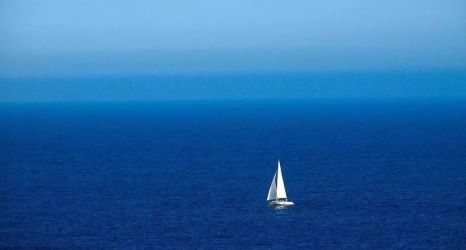
\includegraphics[width=5cm]{1.jpeg}
  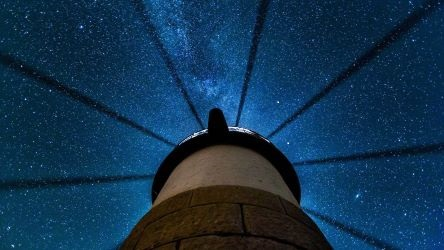
\includegraphics[width=5cm]{2.jpg}
  
\includegraphics[width=5cm]{3.jpg}
  \caption{实验数据集}
  \label{fig:data}
\end{figure}

实验评价指标为: 相同迭代次数下的运行时间, 低秩矩阵的秩, 稀疏噪声矩阵的 0 范数, 以及目标函数值. 具体而言, 鲁棒主成分分析的目标函数值为
\begin{equation}
  f=\|\ml\|_{*}+\lambda\|\ms\|_{m_1},\quad \lambda=\frac{1}{\sqrt{\max(m,n)}},
\end{equation}
矩阵补全的目标函数值为
\begin{equation}
  f=\|\ml\|_{*}.
\end{equation}

\subsection{实验结果分析}

\subsubsection{主成分分析}

主成分分析的实验结果如图 \ref{fig:results_pca}  所示, 其中第 1 行展示了原始图片与添加噪声后的图像, 其余行分别展示了 6 种不同超参数 (\textsf{r0}-\textsf{r5} 分别对应 $\rank(\ml)=[1,2,3,5,10,50]$) 下 PCA 算法的实验结果. 由图 \ref{fig:results_pca} 可知, 随着低秩矩阵秩的增加, 恢复出的低秩图像从仅有模糊背景到较清晰图像再到包含噪声图像逐渐转变, 而噪声图像中的元素逐渐减少趋于空白.

\begin{figure}[!htbp]
  \centering
  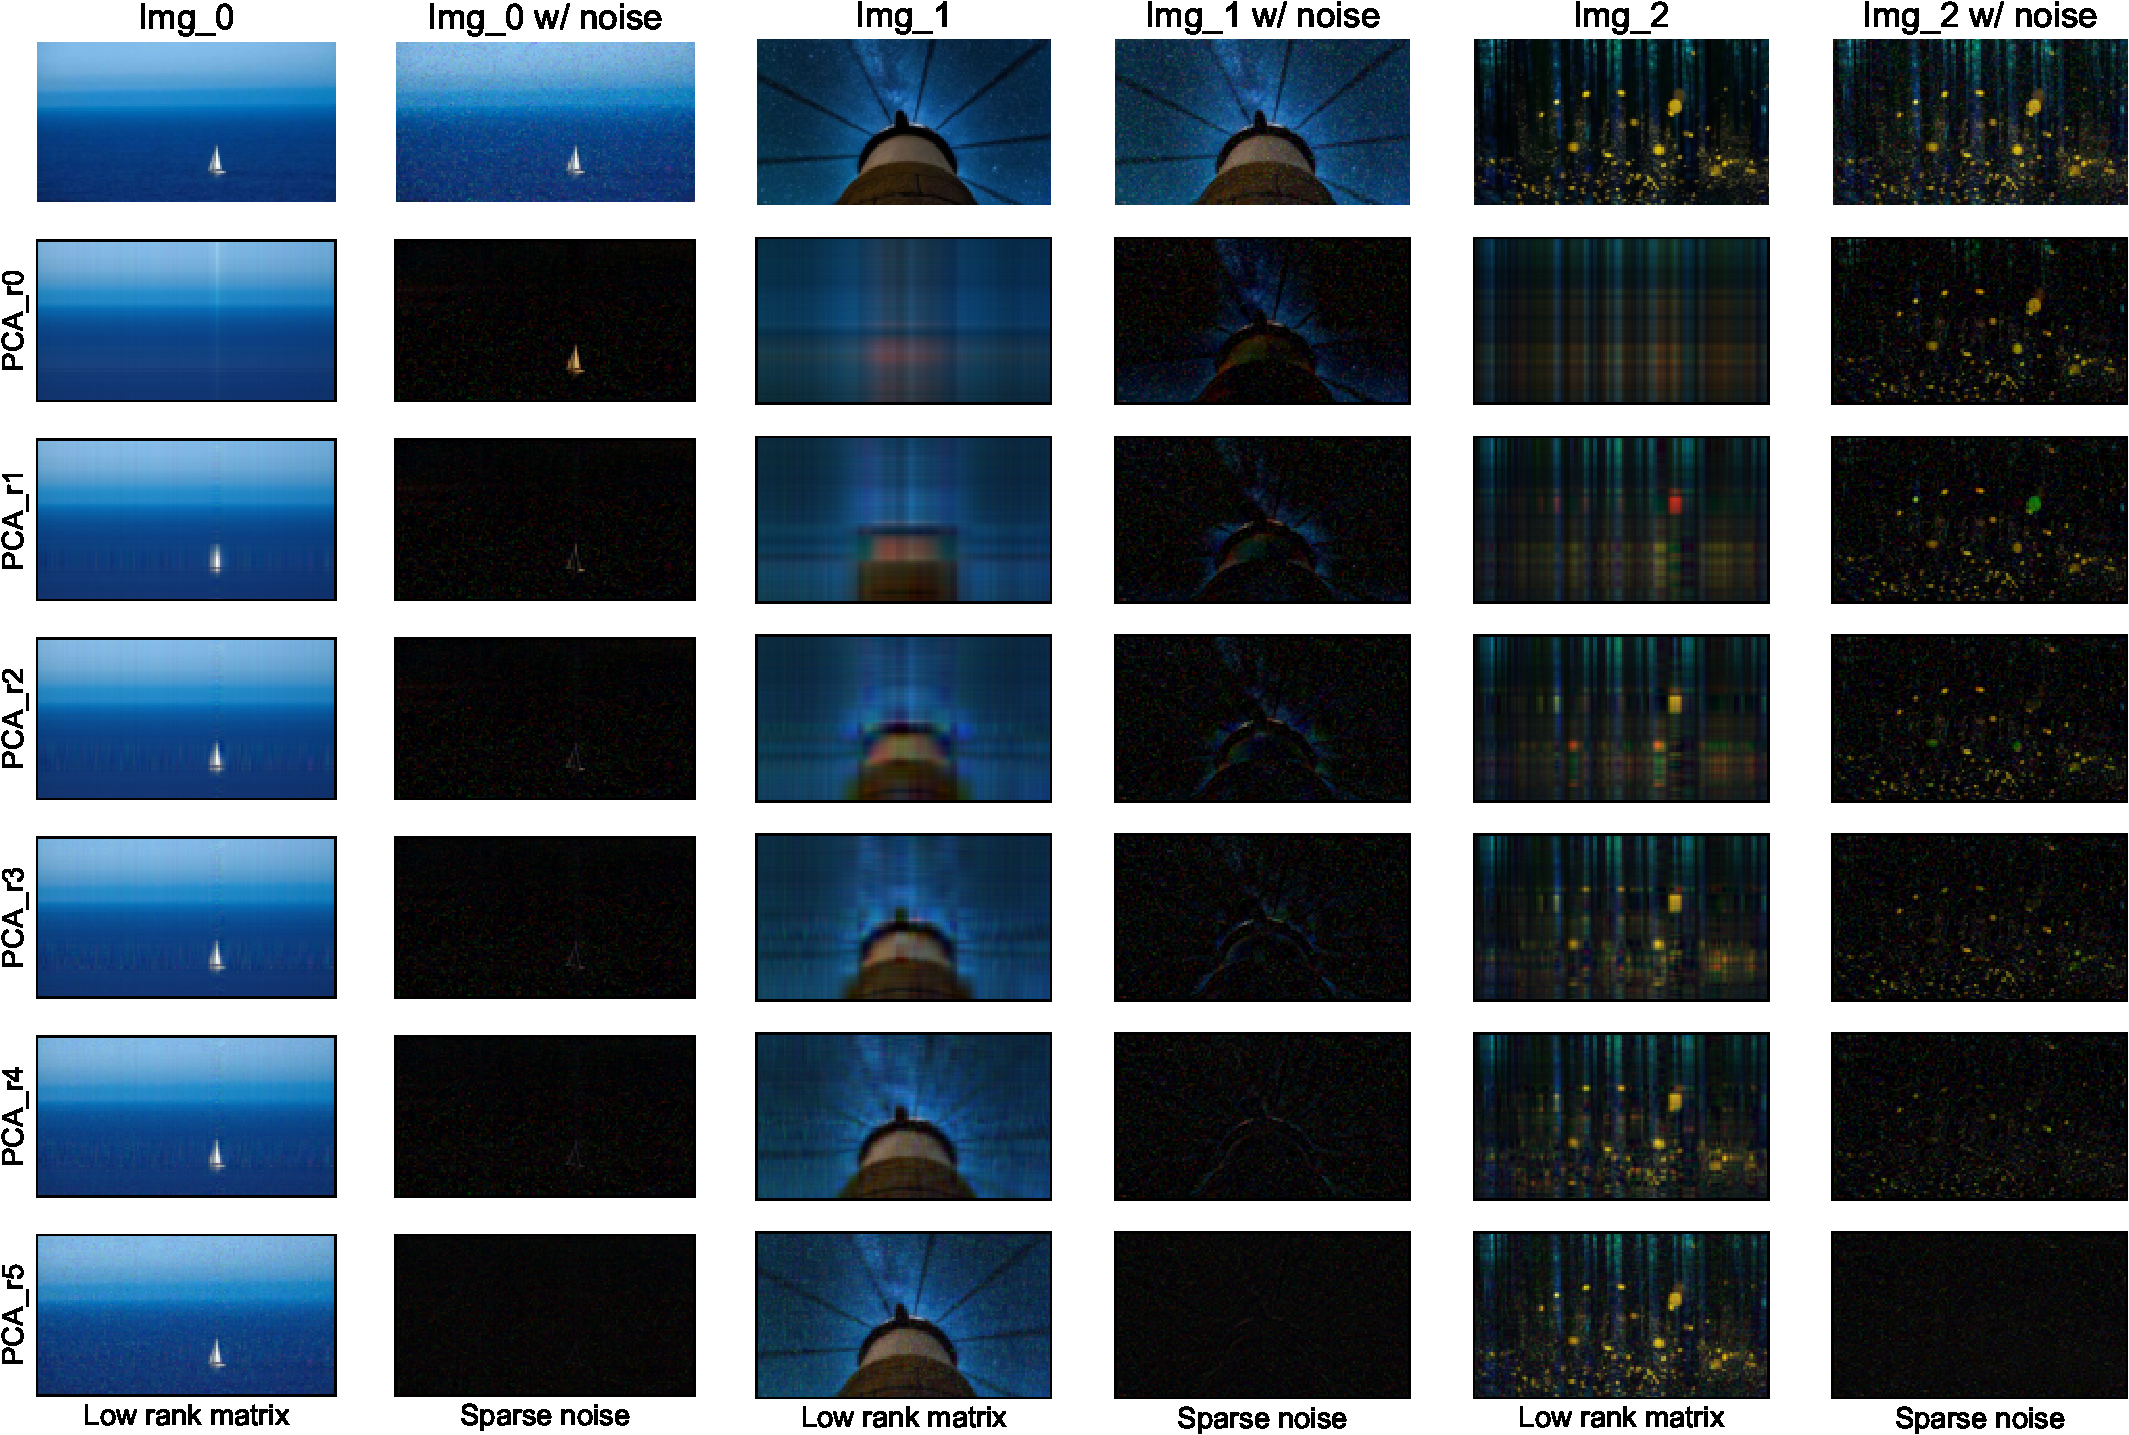
\includegraphics[width=17cm]{pca_total.pdf}
  \caption{主成分分析实验结果}
  \label{fig:results_pca}
\end{figure}

主成分分析算法的性能指标如表 \ref{tab:pca_index} 所示. 由表 \ref{tab:pca_index} 可知, 主成分分析算法所需的运行时间很短, 仅为 0.3 秒, 随着低秩矩阵秩的增加目标函数值先降低再增加.

\begin{table}[!htbp]
  \centering
  \small
  \caption{主成分分析算法性能指标}
  \label{tab:pca_index}
  \begin{tabular}{cccccc}
    \toprule
    Image & Algorithm     & Time (s)  & $\rank(\ml)$ & $\|\ms\|_0$  & $\|\ml\|_{*}+\lambda\|\ms\|_{m_1}$ \\
    \midrule
    0     & PCA r0    & 0.3      & 1.0         & 116500.0    & 398.6         \\
    0     & PCA r1    & 0.3      & 2.0         & 116500.0    & 398.1         \\
    0     & PCA r2    & 0.3      & 3.0         & 116500.0    & 408.5         \\
    0     & PCA r3    & 0.3      & 5.0         & 116500.0    & 428.2         \\
    0     & PCA r4    & 0.3      & 10.0        & 116500.0    & 476.6         \\
    0     & PCA r5    & 0.3      & 50.0        & 116500.0    & 679.1         \\
    1     & PCA r0    & 0.3      & 1.0         & 111000.0    & 570.8         \\
    1     & PCA r1    & 0.3      & 2.0         & 111000.0    & 486.9         \\
    1     & PCA r2    & 0.3      & 3.0         & 111000.0    & 478.5         \\
    1     & PCA r3    & 0.3      & 5.0         & 111000.0    & 475.1         \\
    1     & PCA r4    & 0.3      & 10.0        & 111000.0    & 498.5         \\
    1     & PCA r5    & 0.3      & 50.0        & 111000.0    & 679.6         \\
    2     & PCA r0    & 0.3      & 1.0         & 111000.0    & 514.5         \\
    2     & PCA r1    & 0.3      & 2.0         & 111000.0    & 501.9         \\
    2     & PCA r2    & 0.3      & 3.0         & 111000.0    & 496.9         \\
    2     & PCA r3    & 0.3      & 5.0         & 111000.0    & 502.6         \\
    2     & PCA r4    & 0.3      & 10.0        & 111000.0    & 528.8        \\
    2     & PCA r5    & 0.3      & 50.0        & 111000.0    & 717.7        \\
    \bottomrule
  \end{tabular}
\end{table}

\subsubsection{鲁棒主成分分析}

鲁棒主成分分析的实验结果如图 \ref{fig:results_rpca} 所示, 其中第 1 行展示了原始图片与添加噪声后的图像, 其余行分别展示了 Gradient descent (CGD), Gradient descent with Adam (CGD Adam), Augmented Lagrange multipliers (ALM), Singular value thresholding (SVT), Accelerated proximal gradient (APG) 算法的实验结果. 由图 \ref{fig:results_rpca} 可知, CGD, SVT 和 APG 算法的效果都比较好, ALM 算法在不同超参数下的效果差异比较明显.

\begin{figure}[!htbp]
  \centering
  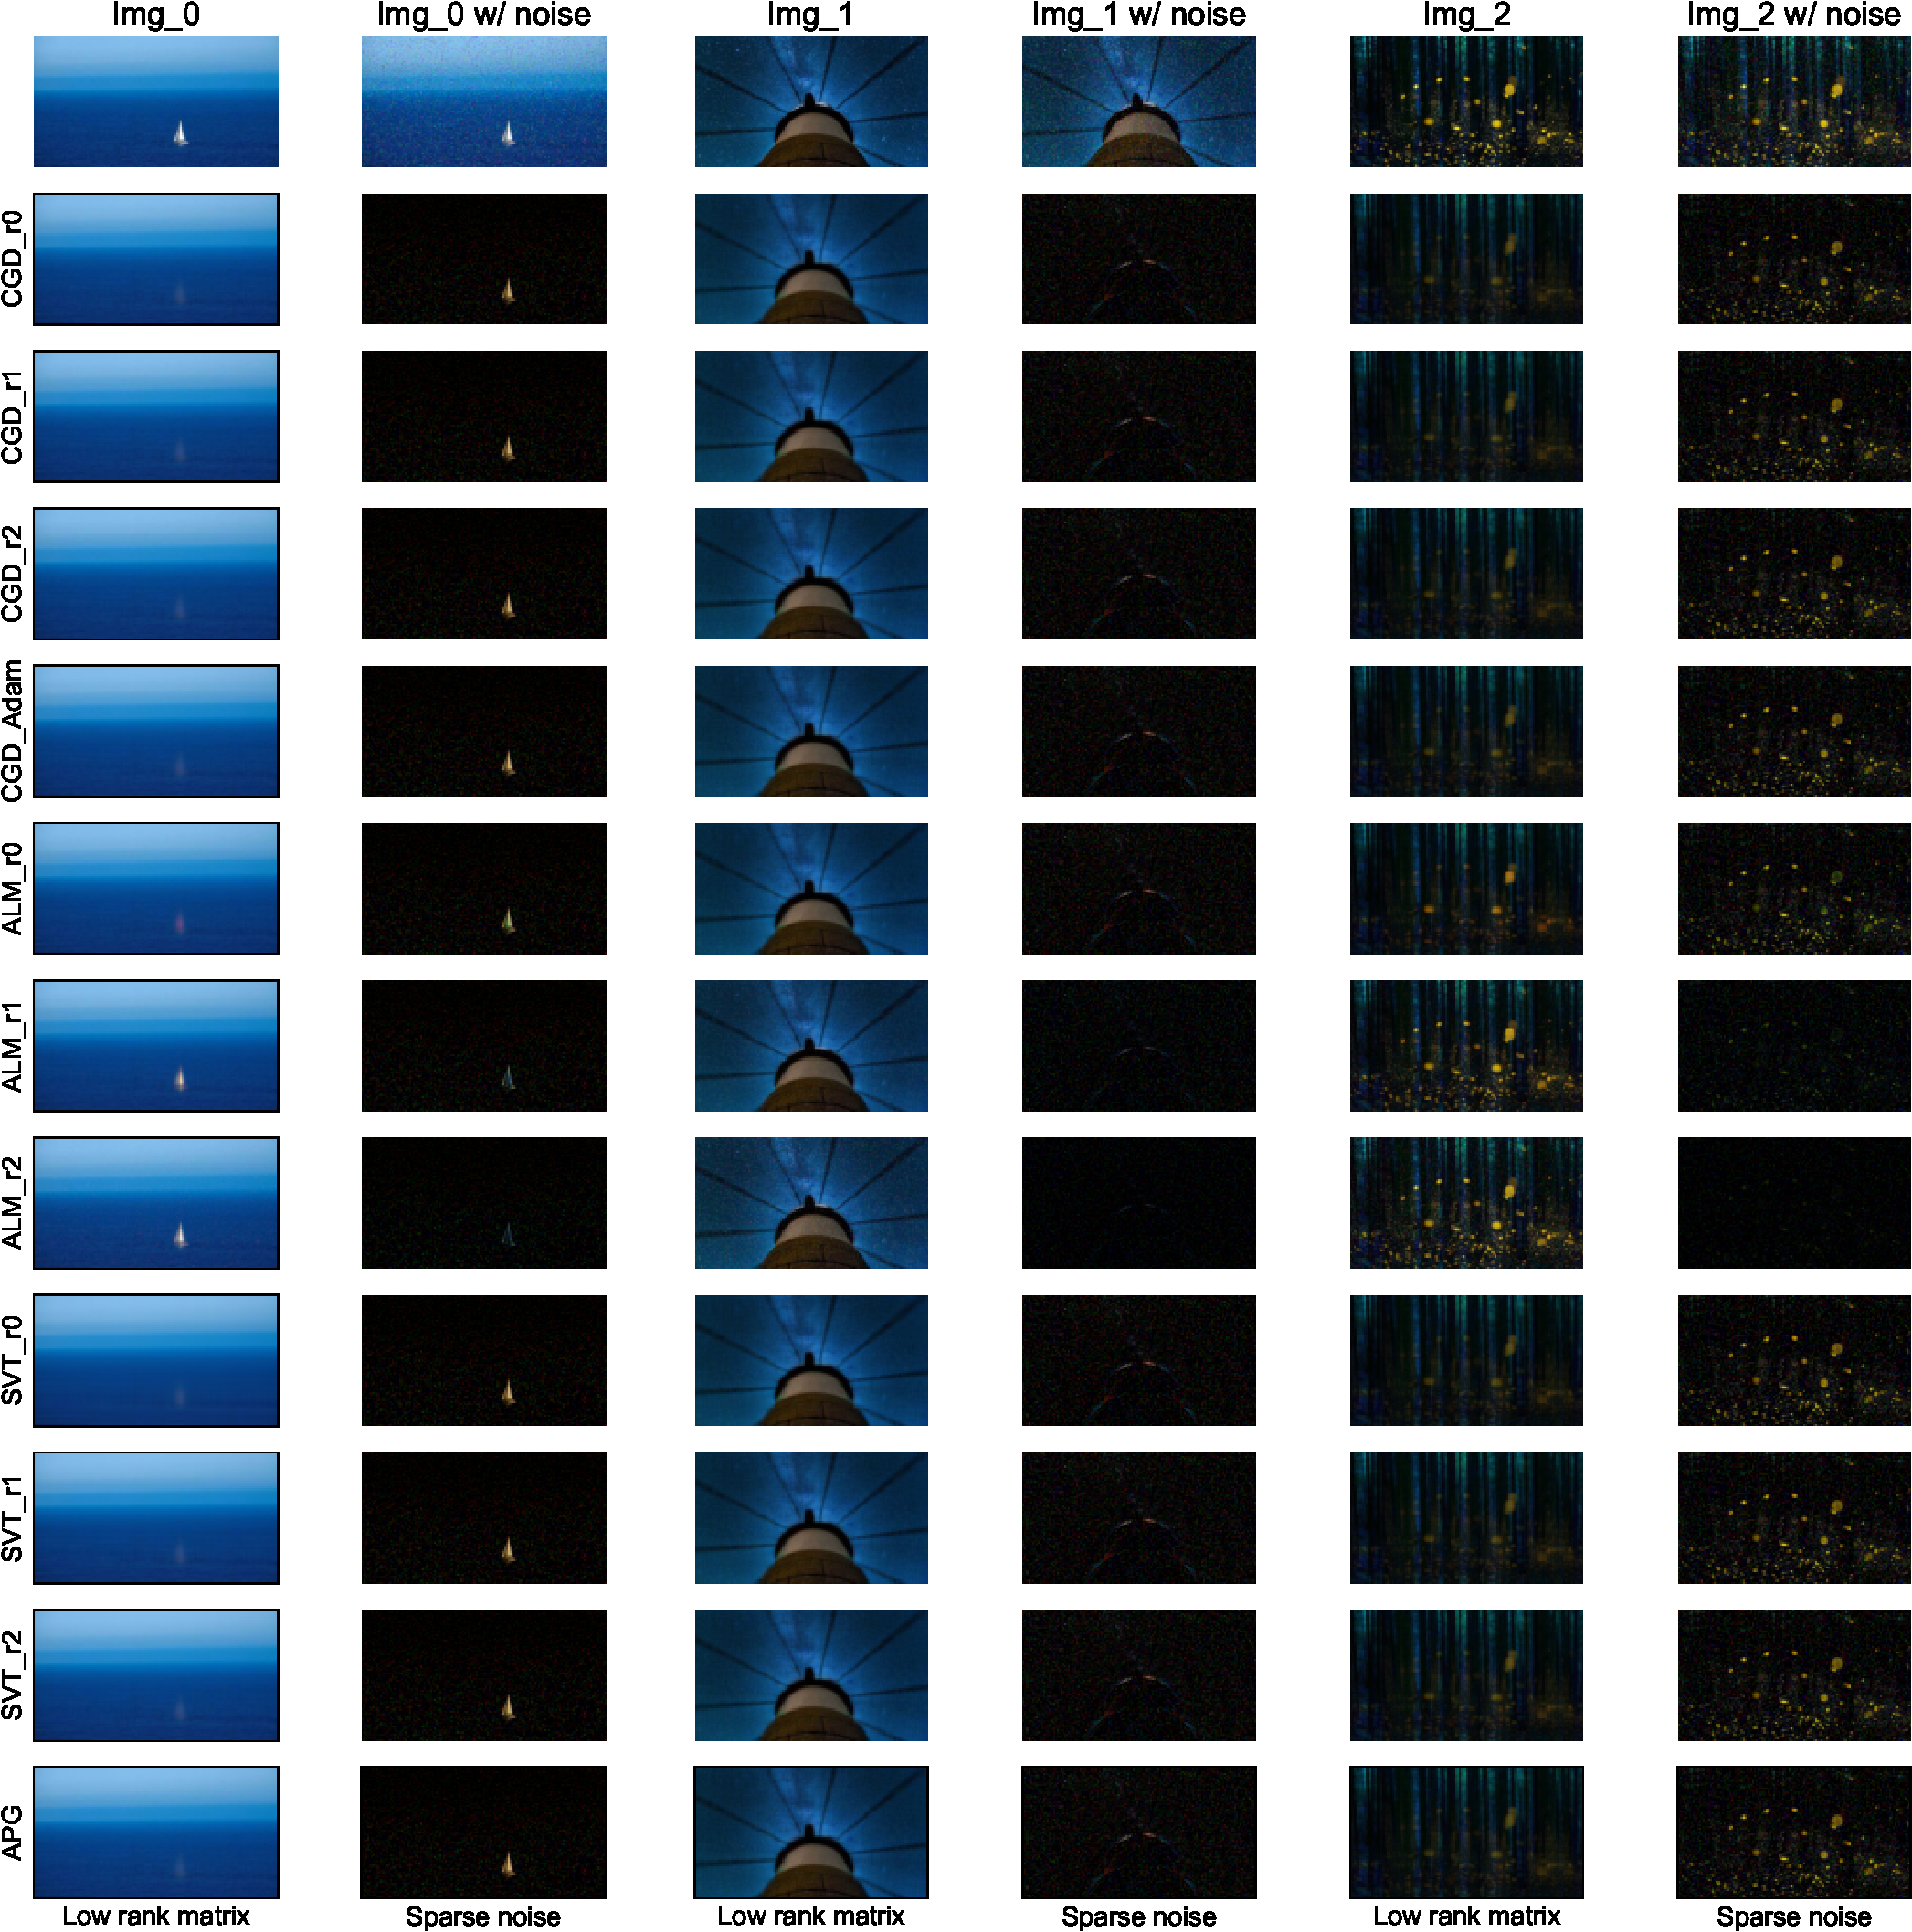
\includegraphics[width=17cm]{robust_pca_total.pdf}
  \caption{鲁棒主成分分析实验结果}
  \label{fig:results_rpca}
\end{figure}

图 \ref{fig:results_rpca} 左侧命名带有 \textsf{r0}, \textsf{r1}, \textsf{r2} 的算法为不同超参数的实验结果, 具体超参数设置如表 \ref{tab:rpca_hyperparams} 所示.

\begin{table}[!htbp]
  \centering
  \small
  \caption{鲁棒主成分分析各算法超参数设置}
  \label{tab:rpca_hyperparams}
  \begin{tabular}{cccc}
    \toprule
    Algorithm  & \textsf{r0}  & \textsf{r1} & \textsf{r2}  \\
    \midrule
    CGD & $\mu\leftarrow0.0005\mu$ & $\mu\leftarrow0.001\mu$ & $\mu\leftarrow0.005\mu$ \\
    ALM & $\mu\leftarrow0.1\mu$ & $\mu\leftarrow0.5\mu$ & $\mu\leftarrow\mu$ \\
    SVT & $\mu=\alpha=0.001$ & $\mu=\alpha=0.002$ & $\mu=\alpha=0.003$ \\
    \bottomrule
  \end{tabular}
\end{table}

鲁棒主成分分析算法的性能指标如表 \ref{tab:rpca_index} 所示. 由表 \ref{tab:rpca_index} 可知, CGD 算法的运行时间显著高于其他 3 个算法, 而且几乎没有达到降秩的结果. 但是 CGD 算法得到的低秩图像和稀疏噪声图像的视觉效果还不错, 所以绝对意义上的降秩并不是达到预期效果的必要条件. SVT 算法的降秩效果最好, 而且噪声矩阵的稀疏性也最好, 因此其目标函数值也是最小的.

\begin{table}[!htbp]
  \centering
  \small
  \caption{鲁棒主成分分析各算法性能指标}
  \label{tab:rpca_index}
  \begin{tabular}{cccccc}
    \toprule
    Image & Algorithm      & Time (s)  & $\rank(\ml)$ & $\|\ms\|_0$    & $\|\ml\|_{*}+\lambda\|\ms\|_{m_1}$ \\
    \midrule
    0     & ALM r0    & 330.7    & 136.3       & 73402.3     & 333.2         \\
    0     & ALM r1    & 329.4    & 141.0       & 72262.0     & 335.3         \\
    0     & ALM r2    & 327.6    & 184.0       & 51798.0     & 385.6         \\
    0     & APG       & 328.0    & 135.7       & 73546.7     & 333.1         \\
    0     & SVT r0    & 322.8    & 4.0         & 6249.3      & 303.3         \\
    0     & SVT r1    & 327.1    & 14.7        & 10840.3     & 313.5         \\
    0     & SVT r2    & 325.6    & 27.7        & 16095.7     & 320.0         \\
    0     & CGD r0    & 535.9    & 250.0       & 116500.0    & 333.2         \\
    0     & CGD r1    & 534.2    & 250.0       & 116500.0    & 333.3         \\
    0     & CGD r2    & 537.1    & 250.0       & 116500.0    & 333.5         \\
    0     & CGD Adam  & 532.9    & 250.0       & 116500.0    & 347.9         \\
    1     & ALM r0    & 260.1    & 140.0       & 72664.0     & 388.1         \\
    1     & ALM r1    & 263.1    & 207.0       & 51589.3     & 425.6         \\
    1     & ALM r2    & 266.7    & 248.0       & 26648.7     & 533.6         \\
    1     & APG       & 262.4    & 141.7       & 73975.7     & 388.1         \\
    1     & SVT r0    & 261.9    & 28.3        & 20876.3     & 335.5         \\
    1     & SVT r1    & 263.6    & 63.7        & 38295.0     & 367.9         \\
    1     & SVT r2    & 265.8    & 85.7        & 48169.7     & 378.1         \\
    1     & CGD r0    & 463.2    & 250.0       & 111000.0    & 388.2         \\
    1     & CGD r1    & 464.9    & 250.0       & 111000.0    & 388.4         \\
    1     & CGD r2    & 466.6    & 250.0       & 111000.0    & 388.6         \\
    1     & CGD Adam  & 468.0    & 250.0       & 111000.0    & 404.4         \\
    2     & ALM r0    & 261.9    & 141.7       & 72063.3     & 374.4         \\
    2     & ALM r1    & 261.2    & 232.3       & 40029.3     & 462.0         \\
    2     & ALM r2    & 268.4    & 250.0       & 19075.7     & 608.6         \\
    2     & APG       & 266.9    & 141.7       & 74387.0     & 373.5         \\
    2     & SVT r0    & 265.1    & 33.7        & 23243.7     & 331.7         \\
    2     & SVT r1    & 263.1    & 58.7        & 36326.7     & 355.5         \\
    2     & SVT r2    & 262.7    & 76.0        & 43697.3     & 363.4         \\
    2     & CGD r0    & 463.7    & 250.0       & 111000.0    & 373.7         \\
    2     & CGD r1    & 465.7    & 250.0       & 111000.0    & 373.9         \\
    2     & CGD r2    & 466.2    & 250.0       & 111000.0    & 374.1         \\
    2     & CGD Adam  & 470.6    & 250.0       & 111000.0    & 395.3        \\
    \bottomrule
  \end{tabular}
\end{table}

\subsubsection{矩阵补全}

矩阵补全的实验结果如图 \ref{fig:results_mc} 所示, 其中第 1 行展示了原始图片与添加噪声后的图像, 其余行分别展示了 Alternating direction method (ADMM), Singular value thresholding (SVT), Alternating least squares (PMF, BPMF) 算法的实验结果. 由图 \ref{fig:results_mc} 可知, ADMM 和 SVT 算法的效果都比较好, PMF 和 BPMF 算法的效果则要差一些.

\begin{figure}[!htbp]
  \centering
  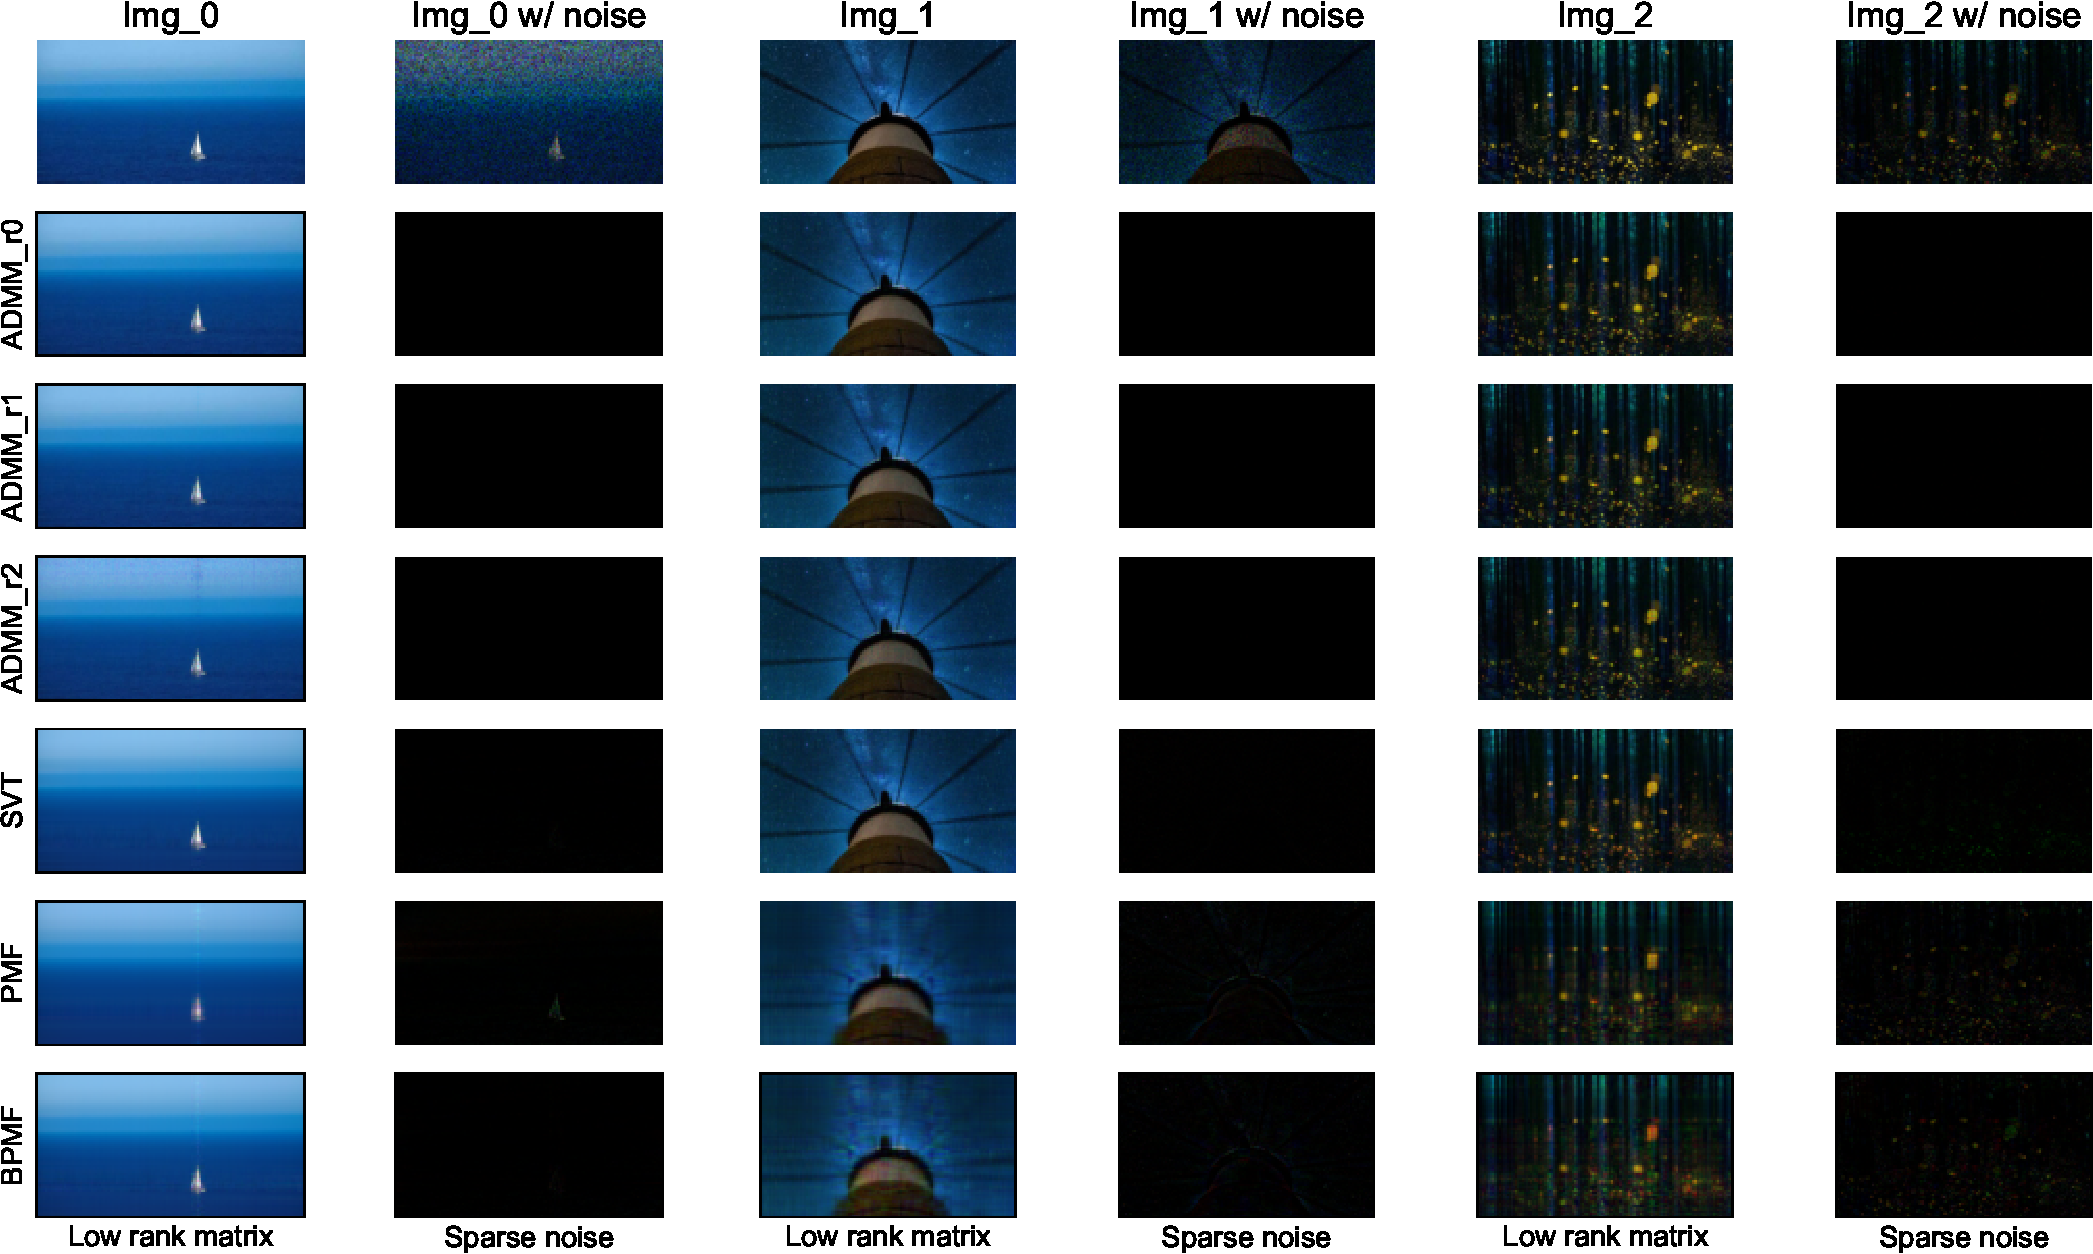
\includegraphics[width=17cm]{matrix_completion.pdf}
  \caption{矩阵补全实验结果}
  \label{fig:results_mc}
\end{figure}

图 \ref{fig:results_mc} 左侧命名带有 \textsf{r0}, \textsf{r1}, \textsf{r2} 的算法为不同超参数的实验结果, 具体超参数设置如表 \ref{tab:mc_hyperparams} 所示.

\begin{table}[!htbp]
  \centering
  \small
  \caption{矩阵补全算法超参数设置}
  \label{tab:mc_hyperparams}
  \begin{tabular}{cccc}
    \toprule
    Algorithm  & \textsf{r0}  & \textsf{r1} & \textsf{r2}  \\
    \midrule
    ADMM & $\mu\leftarrow0.05\mu$ & $\mu\leftarrow0.1\mu$ & $\mu\leftarrow0.15\mu$ \\
    \bottomrule
  \end{tabular}
\end{table}

矩阵补全 CNTK 方法的实验结果如图 \ref{fig:results_mc_ntk} 所示, 其中第 1 行展示了原始图片与添加噪声后的图像, 第 2 行是直接使用 CNTK 方法得到的结果, 第 3 行展示使用 CNTK 和 EigenPro 得到的结果. 由图 \ref{fig:results_mc_ntk} 可知, CNTK 方法得到的结果都比较不错.

\begin{figure}[!htbp]
  \centering
  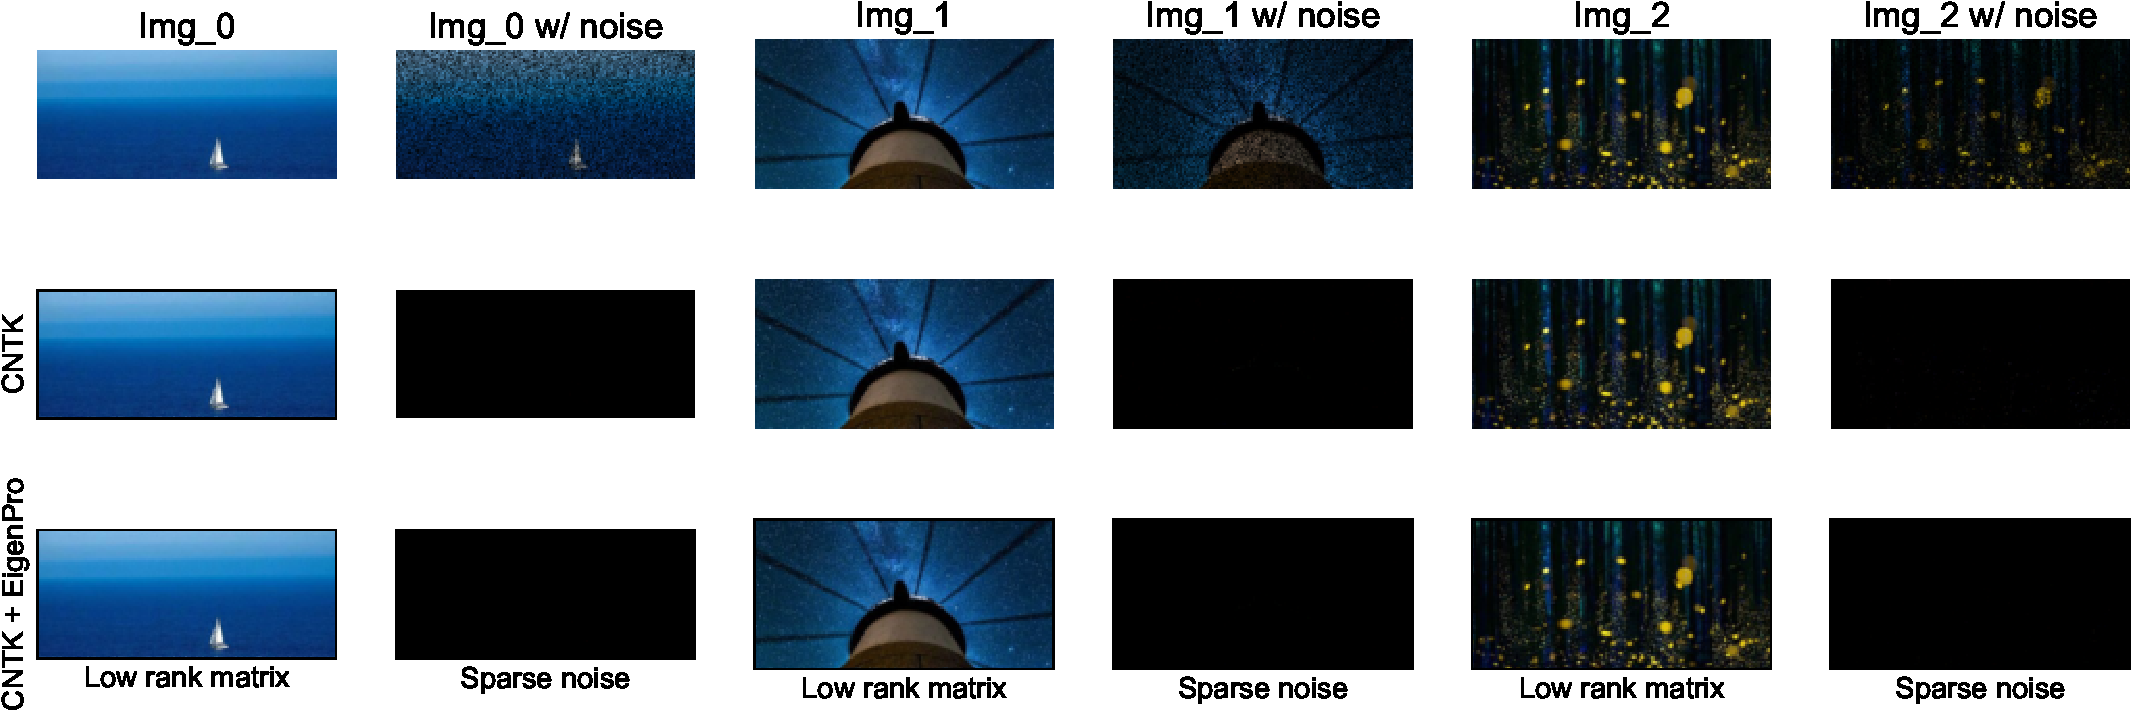
\includegraphics[width=17cm]{matrix_completion_ntk.pdf}
  \caption{矩阵补全 CNTK 方法实验结果}
  \label{fig:results_mc_ntk}
\end{figure}

矩阵补全算法的性能指标如表 \ref{tab:mc_index} 所示. 由表 \ref{tab:mc_index} 可知, ADMM 和 CNTK 算法的运行时间显著多于其他算法, 使用了 EigenPro 的 CNTK 算法的运行时间显著减少. SVT, PMF 和 BPMF 算法得到的低秩矩阵的秩均比较小, 但是噪声矩阵的稀疏性较差.

\begin{table}[!htbp]
  \centering
  \small
  \caption{矩阵补全各算法性能指标}
  \label{tab:mc_index}
  \begin{tabular}{cccccc}
    \toprule
    Image & Algorithm     & Time (s)  & $\rank(\ml)$ & $\|\ms\|_0$  & $\|\ml\|_{*}$ \\
    \midrule
    0     & ADMM r0       & 322.6    & 191.7       & 57822.7     & 206.2         \\
    0     & ADMM r1       & 330.4    & 192.0       & 57822.7     & 206.4         \\
    0     & ADMM r2       & 325.9    & 198.0       & 57822.7     & 239.7         \\
    0     & SVT           & 36.3     & 8.7         & 116500.0    & 178.0         \\
    0     & PMF           & 2.0      & 10.0        & 116500.0    & 164.1         \\
    0     & BPMF          & 2.0      & 12.0        & 116500.0    & 180.7         \\
    0     & CNTK          & 340.7    & 192.0       & 43120.0     & 181.4         \\
    0     & CNTK EigenPro & 69.1     & 192.0       & 43120.0     & 180.0         \\
    1     & ADMM r0       & 263.3    & 196.7       & 53239.3     & 262.9         \\
    1     & ADMM r1       & 266.2    & 200.0       & 53239.3     & 263.7         \\
    1     & ADMM r2       & 261.0    & 205.0       & 53239.3     & 269.6         \\
    1     & SVT           & 297.5    & 58.7        & 111000.0    & 208.4         \\
    1     & PMF           & 1.8      & 10.0        & 111000.0    & 120.6         \\
    1     & BPMF          & 1.9      & 12.0        & 111000.0    & 131.3         \\
    1     & CNTK          & 340.7    & 192.0       & 36756.0     & 238.2         \\
    1     & CNTK EigenPro & 69.1     & 192.0       & 36755.7     & 225.8         \\
    2     & ADMM r0       & 261.5    & 200.7       & 50828.0     & 282.4         \\
    2     & ADMM r1       & 263.2    & 204.0       & 50828.0     & 283.7         \\
    2     & ADMM r2       & 262.5    & 208.0       & 50828.0     & 286.6         \\
    2     & SVT           & 730.6    & 83.3        & 111000.0    & 210.7         \\
    2     & PMF           & 1.9      & 10.0        & 111000.0    & 80.4          \\
    2     & BPMF          & 1.9      & 12.0        & 111000.0    & 95.2          \\
    2     & CNTK          & 340.7    & 192.0       & 36746.0     & 253.3         \\
    2     & CNTK EigenPro & 69.1     & 192.0       & 36746.0     & 236.3        \\
    \bottomrule
  \end{tabular}
\end{table}

\newpage
\section{代码说明}

\subsection{参考代码}

本文参考的代码如表 \ref{tab:code_refs} 所示, 这些代码文件的位置为: \verb|utils/|. 另外, \verb|ntk/| 文件夹为文献 \cite{radhakrishnan2022simple} 作者提供的 CNTK 方法的开源代码, 本文基于该开源代码进行了简单修改, 以用于本任务.

\begin{table}[htbp]
  \centering
  \small
  \caption{参考代码及链接}
  \label{tab:code_refs}
  \begin{tabular}{lll}
    \toprule
    file & function       & link   \\
    \midrule
    \verb|robust_pca.py|    & \verb|_augmented_Lagrange_multipliers()| & \href{https://github.com/dganguli/robust-pca}{Robust-PCA}   \\
    \verb|matrix_completion.py|    & \verb|_singular_value_thresholding()| & \href{https://github.com/tonyduan/matrix-completion}{matrix-completion}   \\
    \verb|matrix_completion.py|    & \verb|_probabilistic_matrix_factorization()| & \href{https://github.com/tonyduan/matrix-completion}{matrix-completion}   \\
    \verb|matrix_completion.py|    & \verb|_biased_probabilistic_matrix_factorization()| & \href{https://github.com/tonyduan/matrix-completion}{matrix-completion}   \\
    \bottomrule
  \end{tabular}
\end{table}

\subsection{代码结构}

代码结构如表 \ref{tab:code_framework} 所示, 其中核心算法位于 \verb|utils/| 文件夹.

\begin{table}[htbp]
  \centering
  \small
  \caption{代码结构}
  \label{tab:code_framework}
  \begin{tabular}{lll}
    \toprule
    folder & description    \\
    \midrule
    \verb|bin/|    &  testing algorithms, analyzing results, and plotting figures   \\
    \verb|data/|    &  source data and results   \\
    \verb|doc/|    &  documentation   \\
    \verb|ntk/|    &  the CNTK algorithm   \\
    \verb|pre/|    &  slides   \\
    \verb|utils/|    &  algorithms   \\
    \bottomrule
  \end{tabular}
\end{table}

\section{贡献说明}

本研究的分工如表 \ref{tab:contribution} 所示.

\begin{table}[htbp]
  \centering
  \small
  \caption{贡献说明}
  \label{tab:contribution}
  \begin{tabular}{lll}
    \toprule
    工作内容 & 完成人    \\
    \midrule
    鲁棒主成分分析: 通用算法 & 杨敬轩 \\
    鲁棒主成分分析: 特殊算法 & 杨敬轩 \\
    矩阵补全算法 & 董泽委 \\
    实验结果分析 & 杨敬轩, 董泽委 (1: 0.9) \\
    报告撰写 & 杨敬轩, 董泽委 (1: 0.7) \\
    Beamer 制作 & 杨敬轩, 董泽委 (1: 0.5) \\
    \bottomrule
  \end{tabular}
\end{table}

\section{结论}

本文针对低秩矩阵恢复问题进行探究, 主要研究了鲁棒主成分分析算法以及矩阵补全算法. 针对鲁棒主成分分析算法, 给出了基于梯度下降算法的通用求解方法, 并基于 Adam 算法进行优化, 然后给出了 3 种特殊优化算法: SVT, APG 与 ALM. 针对矩阵补全问题, 给出了矩阵补全问题的数学模型, 以及 4 种具体求解算法: SVT, ADMM, ALS, CNTK. 本文对上述算法在图像数据集上的效果进行了测试, 结果表明 PCA 算法的求解时间最短, 但是效果比较一般, 鲁棒主成分分析算法的效果更好, 但是耗时普遍较长, 其中 SVT 算法的用时较短且取得了相对更好的效果; 矩阵补全算法也可以实现低秩矩阵恢复, ADMM 和 SVT 算法的效果均比较好但用时较长, CNTK 算法效果较好, 若与 EigenPro 联合使用可以达到用时少与效果好的双重目的. 本文还对不同超参数的实验结果进行了测试和分析.

\setlength{\bibsep}{1.5pt}
\bibliographystyle{unsrt}
\addcontentsline{toc}{section}{参考文献}
\bibliography{ref.bib}

\end{document}
